\section{Introduction}

As the power of AI increases, it is of increasing desire to apply
it in ways to augment the decision making processes. This process
may include just a singular human, or that it might involve
multiple people. As the number of people change, and even the
domain itself changes, so too does the environment.

In contemporary AI research devoted to decision support, the challenge
is often taken to be that of providing AI support to a single human.
However, much human problem solving
is fundamentally social, in that a group of people must work together
to solve a problem, and must rely upon machine intelligence that is
itself highly diverse.  Examples of such activities include: hiring a
person into a university or company, tackling an emergency crisis like
a major water pipeline break, planning an intricate medical operation,
and deciding which companies to merge with or acquire.  Motivated by
such challenges, we are interested in how an artificial agent ---
embedded in a social-collaboration environment like an immersive room
--- can, on the spot, help a group of human participants.

%%%%%%%%%%%%%%%%%%%%%%%%%%%%%%%%%%%%%%%%%%%%%%%%%%%%%%%%%%%%%%%%%%%%%%
\begin{figure}
\centering
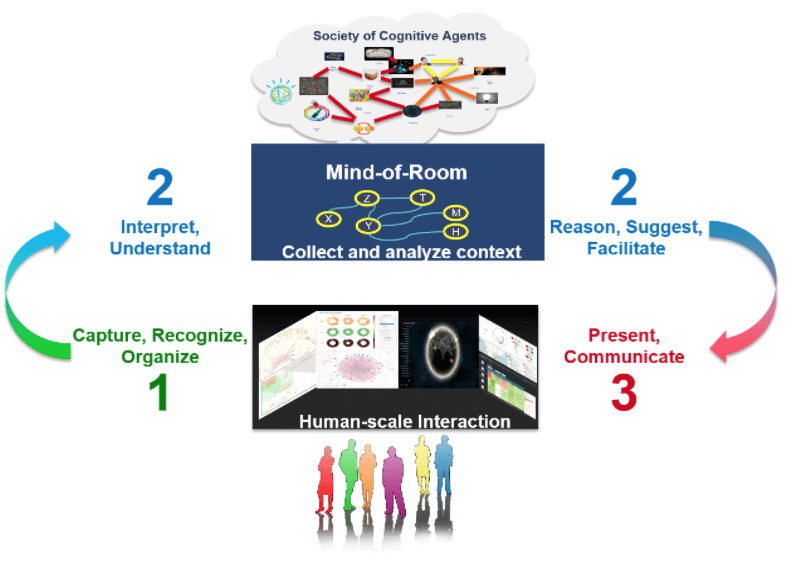
\includegraphics[width=0.5\columnwidth]{chapters/01_introduction/figures/cisl-cycle-graphic.png}
\caption{The flow of information through the elements of a cognitive and immersive system.}
\label{fig:cycle-cais}
\end{figure}
%%%%%%%%%%%%%%%%%%%%%%%%%%%%%%%%%%%%%%%%%%%%%%%%%%%%%%%%%%%%%%%%%%%%%%

We first introduce the notion of a \emph{cognitive and immersive
  system} (CAIS), which comprises three elements linked in a cyclical
flow as shown in Figure \ref{fig:cycle-cais}.  The first element is
responsible for perception and sensing within the environment that
contains the human agents (specifically, here, within a room).
Percepts come courtesy of a range of sensors, such as microphones and
kinects.  The second element interprets, understands, and acts upon
perceived data through reasoning, planning, learning, and language.
The third element displays both percepts and the results of processing
these percepts in rich, multi-modal ways.  The particular CAIS we have
used for our investigations
%% ``The CAIS''
%
%% MATT: It doesn't make any sense to refer to /the/ CAIS unless we
%% have given it a proper name, etc.  We need a proper
%% name/designator.  As far as I can see, there hasn't been a proper
%% name cooked up to refer to a particular CAIS around which CISL work
%% has centered. //S
also has access to external machines and services that can process
requests, queries, and tasks; and this CAIS can incorporate the
results of its analysis of such information into subsequent decision
making.  An important part of our system is that there are overseeing
AIs (agents) operating at the system level that can use the rest of
the system to assist and aid the humans and other AIs that are
operating within the room.  Thus, the overarching architecture is
neither fully centralized nor fully distributed, but aims to combine
the strengths of both.

As an initial test of our CAIS architecture, we implement and examine
two scenarios in which participants have an imbalance of knowledge and
beliefs, and how their their individual beliefs influence their actions.
%% MATT2: What would be doing the influencing?  The imbalance itself?
%% Or the knowledge and beliefs themselves?  I think you need to go
%% through the entire paper with an eye to this kind of ambiguity,
%% because actually the one here isn't the first.  I tried to fix the
%% prior ones.  Thx.  //S
It is common in group discussions that not all participants are aware
of everything said, whether because they missed something or
misconstrued it.  Thus participants may try to act on beliefs of
theirs that do not properly reflect reality, or they may know of their
ignorance and wish to remedy it.  A CAIS should be able to offer help
to participants in these cases, either by alerting them if they are
acting on beliefs that are no longer relevant or right, or by
summarizing what happened while they were out of the discussion.  To
do this, the system must have a theory of the minds
\cite{premack_does_1978,frith_theory_2005,arkoudas_propositional_2009} of participants
and must track and adjust such theories through time.  On the basis of
this modeling, the system must
%% then synthesize this for the agents, and must understand how it
%% relates to their actions and
step in as necessary to offer corrective advice, along with
justifications for doing so.  Most important for us is that the
particular capacities we have just enumerated as desiderata not be
\textit{ad hoc}; the need for these capacities must flow from
underlying formal requirements.

To accomplish the above tasks, we first present informal requirements
that differentiate a CAIS from other intelligent agents.  We state
these requirements in terms of the cognitive states and common
knowledge of the participating agents.  As far as we know, this is the
first characterization of what separates an intelligent room from an
intelligent agent.  We then cast the informal requirements in formal
computational logic and show that these requirements, thus sharpened,
lead to a useful property.  Next, we briefly present a framework for
problems that can be used to test a CAIS, define two tests within that
framework, and show that via this property the system solve the tests
in question.  Finally, we discuss related research, clarify the unique
power of our approach, we discuss promising future lines of work.
